\chapter{Evaluation} \label{chapter:evaluation}
This chapter describes the evaluation of the proposed approach. The evaluation is based on a user study, which is described in detail in Appendix \ref{appendix:evaluation-protocol}. The results of the user study are presented in section \ref{sec:evaluation:results}.

\section{Methodology} \label{sec:evaluation:methodology}
The evaluation was conducted as a controlled user study to assess the effect of the proposed system on robotic program comprehension and modification compared to the baseline workflow. The baseline condition used UR Studio, a browser-based PolyScope X simulation tool from Universal Robots with a visual programming interface similar to programming on the teach pendant.

The study addressed four research questions:
\begin{adjustwidth}{\indentWidthTwenty}{\indentWidthTwenty}
    \textit{\textbf{RQ1:} How does the proposed system influence the correctness of comprehension of robotic programs?}
\end{adjustwidth}
\begin{adjustwidth}{\indentWidthTwenty}{\indentWidthTwenty}
    \textit{\textbf{RQ2:} How does the proposed system influence the time required for comprehension of robotic programs?}
\end{adjustwidth}
\begin{adjustwidth}{\indentWidthTwenty}{\indentWidthTwenty}
    \textit{\textbf{RQ3:} How does the proposed system influence the correctness of modification and reuse of robot programs?}
\end{adjustwidth}
\begin{adjustwidth}{\indentWidthTwenty}{\indentWidthTwenty}
    \textit{\textbf{RQ4:} How does the proposed system influence the time required in the modification and reuse of robot programs?}
\end{adjustwidth}

\subsection{Study Design}
The experiment used a within-subjects design in which each participant completed tasks in both conditions (baseline and proposed system). To reduce order effects, condition order was counterbalanced across participant groups. In addition, two distinct task sets were used across conditions so that participants could not directly transfer solutions from one condition to the other.

Each condition consisted of two phases:
\begin{itemize}
    \item \textbf{Exploration phase:} Participants first familiarized themselves with the assigned condition through guided walkthroughs and practice.
    \item \textbf{Task phase:} Participants then completed comprehension and modification tasks used for evaluation.
\end{itemize}

\subsection{Participants and Pre-Study Survey}
Participants were recruited from potential users of the system, including robotics engineers and programmers with experience in robotic systems, sourced from industry and academia. Before starting the tasks, each participant completed a pre-study survey capturing self-reported robotic programming experience and familiarity/use of AI assistants.

\subsection{Task Design}
The task set was designed to reflect realistic work with robot programs and to evaluate both understanding and change implementation.

Comprehension tasks required participants to inspect programs and answer multiple-choice questions on key actions, action order, waypoint order, URCap usage, gripper usage, and the overall application. Participants also rated their confidence in their own comprehension on a 1--5 Likert scale.

Modification tasks required participants to apply concrete changes to existing programs. Across the two task sets, these changes included modifying speed, changing movement type, switching waypoints between move actions, enabling blend movement, and adding a wait action.

\subsection{Metrics}
The evaluation combined quantitative and qualitative metrics.

Quantitative metrics were:
\begin{itemize}
    \item \textbf{Correctness of comprehension:} Number of correctly answered comprehension questions.
    \item \textbf{Time for comprehension:} Time required to complete comprehension tasks.
    \item \textbf{Correctness of modifications:} Degree to which implemented changes satisfied task requirements, including preservation of existing functionality where applicable.
    \item \textbf{Time for modifications:} Time required to complete modification tasks.
    \item \textbf{Confidence ratings:} Post-task confidence on a 1--5 Likert scale.
\end{itemize}

For comprehension, correctness was based on correct multiple-choice responses. For modification, correctness was evaluated against predefined expected outcomes, with partial correctness assigned when only part of the required change was achieved.

Qualitative metrics were:
\begin{itemize}
    \item System-wide user feedback on usability, usefulness, and challenges.
    \item Feedback specifically on LLM-assisted functionality (user perceived response quality, relevance, clarity, and factual correctness).
    \item Observational data on participant behavior, interactions, and encountered difficulties.
\end{itemize}

\subsection{Procedure}
For each participant, the study proceeded as follows: (1) pre-study survey, (2) completion of the two conditions in counterbalanced order, with an exploration phase followed by a task phase in each condition, and (3) post-study questionnaire.

After completing the tasks, participants provided post-study ratings on ease of use, perceived usefulness, confidence in comprehension and modification for both conditions, and assessments of LLM-generated comprehension responses and modification suggestions. Open-ended questions captured perceived challenges, improvement suggestions, and willingness to use the proposed system in future robotic programming work.

This procedure enabled direct comparison of correctness, completion time, confidence, and user experience between the proposed system and the baseline approach while controlling for learning effects through counterbalancing and distinct task sets.


\section{Results} \label{sec:evaluation:results}
This section presents the results of the user study collected from five participants. Condition A denotes the baseline (UR Studio) and condition B denotes the system proposed in this thesis. The raw evaluation results used in this analysis are provided in Appendix \ref{appendix:evaluation-data}.

The evaluation was performed on with the following hardware; CPU: AMD Ryzen 7 9800X3D, RAM: 32GB DDR5, GPU: NVIDIA RTX 5070 Ti. Language models as described in Chapter \ref{chapter:implementation}.

\subsection{Data Preparation}
Correctness scores for comprehension tasks were scored as 1 for correct and 0 for incorrect answers.

\textbf{Comprehension Task (CT):}
\begin{itemize}
    \item \textbf{CT-1 (Key Actions)}
    \item \textbf{CT-2 (Action Sequence)}
    \item \textbf{CT-3 (Waypoint Sequence)}
    \item \textbf{CT-4 (URCap Usage)}
    \item \textbf{CT-5 (Gripper Type)}
    \item \textbf{CT-6 (Overall Application)}
\end{itemize}

For modification tasks, correctness was scored based on the degree to which the implemented change met the task requirements, with partial credit assigned for partially correct solutions. All programs were verified with UR Studio and manual code analysis. The scoring rubric for modification tasks was as follows:

\textbf{Modification Task (MT) Scoring Rubric:}
\begin{itemize}
    \item \textbf{MT-1 (Speed Modification):} Correctly changing the "optiMoveSpeed" parameter scores 1 point; changing the other speed parameter scores 0 points.
    \item \textbf{MT-2 (Movement Type Change):} Changing the "moveType" from moveL to moveJ or vice versa scores 1 point; no change or an incorrect change scores 0 points.
    \item \textbf{MT-3 (Waypoint Switch):} Correctly switching the positions of the waypoints in the correct order and with the correct move type and parameters scores 1 point; any other change scores 0 points.
    \item \textbf{MT-4 (Blend Enablement):} Enabling blend without specifying a blend radius scores 0.5 points; enabling blend with a specified blend radius scores 1 point; not enabling blend or incorrect changes score 0 points.
    \item \textbf{MT-5 (Wait Node Addition):} Inserting a wait node with the correct structure and in the correct spot scores 1 point; any other change scores 0 points.
\end{itemize}

\subsection{Pre-Study Participant Profile}
The pre-study responses provide context for interpreting the task results. Regarding robotics-programming experience, three participants reported \textit{Intermediate} experience (60\%), one reported \textit{Beginner} (20\%), and one reported \textit{Advanced} (20\%). Thus, all participants had at least some experience with robotic programming, with a majority at the self-proclaimed intermediate level.

For general software-development work, four participants reported frequent AI-assistant usage: two \textit{Always} (40\%) and two \textit{Often} (40\%), while one reported \textit{Sometimes} (20\%). All participants where familiar with AI assistants for software development, with the majority using them frequently.

All participants were positively inclined toward AI assistance for robot program development before the study: three selected \textit{Strongly agree} (60\%) and two selected \textit{Agree} (40\%) for the statement that they would use an AI assistant for developing robot programs.

The participants were asked to explain their reasoning to why or why not to use AI for robot program development. Participants primarily emphasized productivity and acceleration benefits, such as reducing integration time, receiving solution suggestions during development, and faster drafting of robot programs. One participant also highlighted a potential trade-off, noting concern that heavy AI use could reduce deeper understanding of the robot program if the assistant "does everything". Overall, pre-study attitudes suggest optimism: participants expected AI assistance to be useful, while still recognizing possible impacts on learning depth.


\subsection{Quantitative Results}
All participants completed both conditions. Some participants gave up on certain modification subtasks, with one value marked \textit{DNF} (Did Not Finish) in condition A and four values marked \textit{DNF} in condition B.

For consistency, all reported task-time means and medians are computed from completed tasks only, while \textit{DNF} cases are accounted for separately through the task-completion-rate metric.

For correctness, two metrics are reported: (1) completed-only correctness (excluding \textit{DNF} values), and (2) DNF-inclusive correctness where \textit{DNF} is treated as incorrect. In the summary table, DNF-inclusive values are shown in parentheses after completed-only values.

The participants had the option to use the AI assistant in condition B as much or as little as they wanted. Some participants only used the assistant when they were blocked, while others used it more proactively to explore functionality. Thus, the subjective assistant usage is an important factor to consider when interpreting the results.

Assistant interaction logs were collected for 43 assistant requests across all participants. Each log includes a session start and end timestamp, where start is the user query and end is the assistant's final response. The manually extracted file \texttt{assistant\_task\_extraction.csv} links each assistant session with a \texttt{task\_id} label.

Table \ref{tab:evaluation:key-results} summarizes the primary quantitative outcomes.

\begin{table}[H]
    \centering
    \begin{tabular}{p{7cm}cc}
        \toprule
        \textbf{Metric}                          & \textbf{Baseline (A)} & \textbf{Proposed (B)} \\
        \midrule
        Comprehension correctness                & 1.00 (1.00)           & 0.97 (0.97)           \\
        Modification correctness                 & 1.00 (0.96)           & 0.60 (0.50)           \\
        Comprehension time, mean [min]           & 3.25                  & 6.97                  \\
        Comprehension time, median [min]         & 2.62                  & 6.18                  \\
        Modification time, mean [min]            & 4.85                  & 9.81                  \\
        Modification time, median [min]          & 4.03                  & 12.53                 \\
        Comprehension task completion rate       & 1.00                  & 1.00                  \\
        Modification task completion rate        & 0.96                  & 0.84                  \\
        Confidence in comprehension (Likert 1-5) & 4.40                  & 2.00                  \\
        Confidence in modification (Likert 1-5)  & 3.40                  & 2.60                  \\
        \bottomrule
    \end{tabular}
    \caption{Quantitative result summary across baseline (A) and proposed (B) conditions. For correctness rows, values in parentheses are DNF-inclusive (\textit{DNF}=incorrect). Time means/medians are based on completed tasks only; \textit{DNF} cases are reflected in the completion-rate rows.}
    \label{tab:evaluation:key-results}
\end{table}

\subsubsection*{RQ1: How does the proposed system influence the correctness of comprehension of robotic programs?}
The proposed system had a negligible effect on comprehension correctness. Scores were near-perfect in both conditions: baseline reached proportion correct of 1.00 (30/30), and the proposed condition achieved 0.97 (29/30). The single incorrect response in the proposed condition occurred on the action-sequence task, where one participant chose the wrong action chain. This is the strongest positive result for the proposed system. Even with the raw \texttt{.urpx} representation of the program, participants were generally able to identify key actions, action order, waypoint order, URCap usage, gripper type, and overall program application. The structured JSON view, combined with the program tree navigation panel and assistant explanations, was sufficient to support correct program comprehension at the level required by these tasks.

\subsubsection*{RQ2: How does the proposed system influence the time required for comprehension of robotic programs?}
The proposed system increased wall-clock comprehension time. Mean comprehension time per participant increased from 3.25 for the baseline to 6.97 minutes for the proposed system, a roughly 2x increase. The median followed the same pattern, increasing from 2.62 to 6.18 minutes. The paired Wilcoxon test gave $p = 0.31$ ($n=5$), and Cliff's delta was $\delta = +0.52$. This means that, with this sample size, the statistical test does not indicate a reliable difference at conventional significance levels, but the effect-size estimate suggests a practically large shift toward longer comprehension times in the proposed condition.

When assistant wait time is subtracted, the interpretation changes. The mean active comprehension time (subtracting assistant wait time) in the proposed condition was 4.07 minutes, and the effect size dropped to $\delta = +0.20$. This indicates that most of the observed wall-clock increase came from assistant latency rather than substantially slower user work.

The task-level breakdown in Figure \ref{fig:evaluation:time-by-task-ai-comp} is consistent with this interpretation when the proposed mean is split by assistant use. For CT-1, CT-2, CT-4, and CT-5, the proposed \textit{without-assistant} means were close to baseline (CT-1: $-16.5$ s, CT-2: $-11.9$ s, CT-4: $+0.7$ s, CT-5: $+3.6$ s), and CT-6 was faster than baseline ($-47.7$ s). In contrast, the proposed \textit{with-assistant} means were markedly higher than baseline on most tasks (CT-1: $+186.0$ s, CT-2: $+175.6$ s, CT-3: $+201.0$ s, CT-4: $+150.5$ s, CT-5: $+61.6$ s). CT-3 remained slower even without assistant use ($+27.5$ s), suggesting additional task-intrinsic difficulty for waypoint-sequence tracing in the raw JSON representation.

Assistant logs show the same pattern for comprehension-task sessions. Across 24 comprehension-linked sessions, mean response time was 40.94 s (median 40.94 s). Mean embedding time was 4.16 s per call. The 5-call retrieval cap was reached in 8.3\% of comprehension sessions (2/24), and those capped sessions averaged 62.48 s. Together, this suggests that reducing assistant latency is likely to reduce a large portion of the comprehension-time penalty.

\begin{figure}[H]
    \centering
    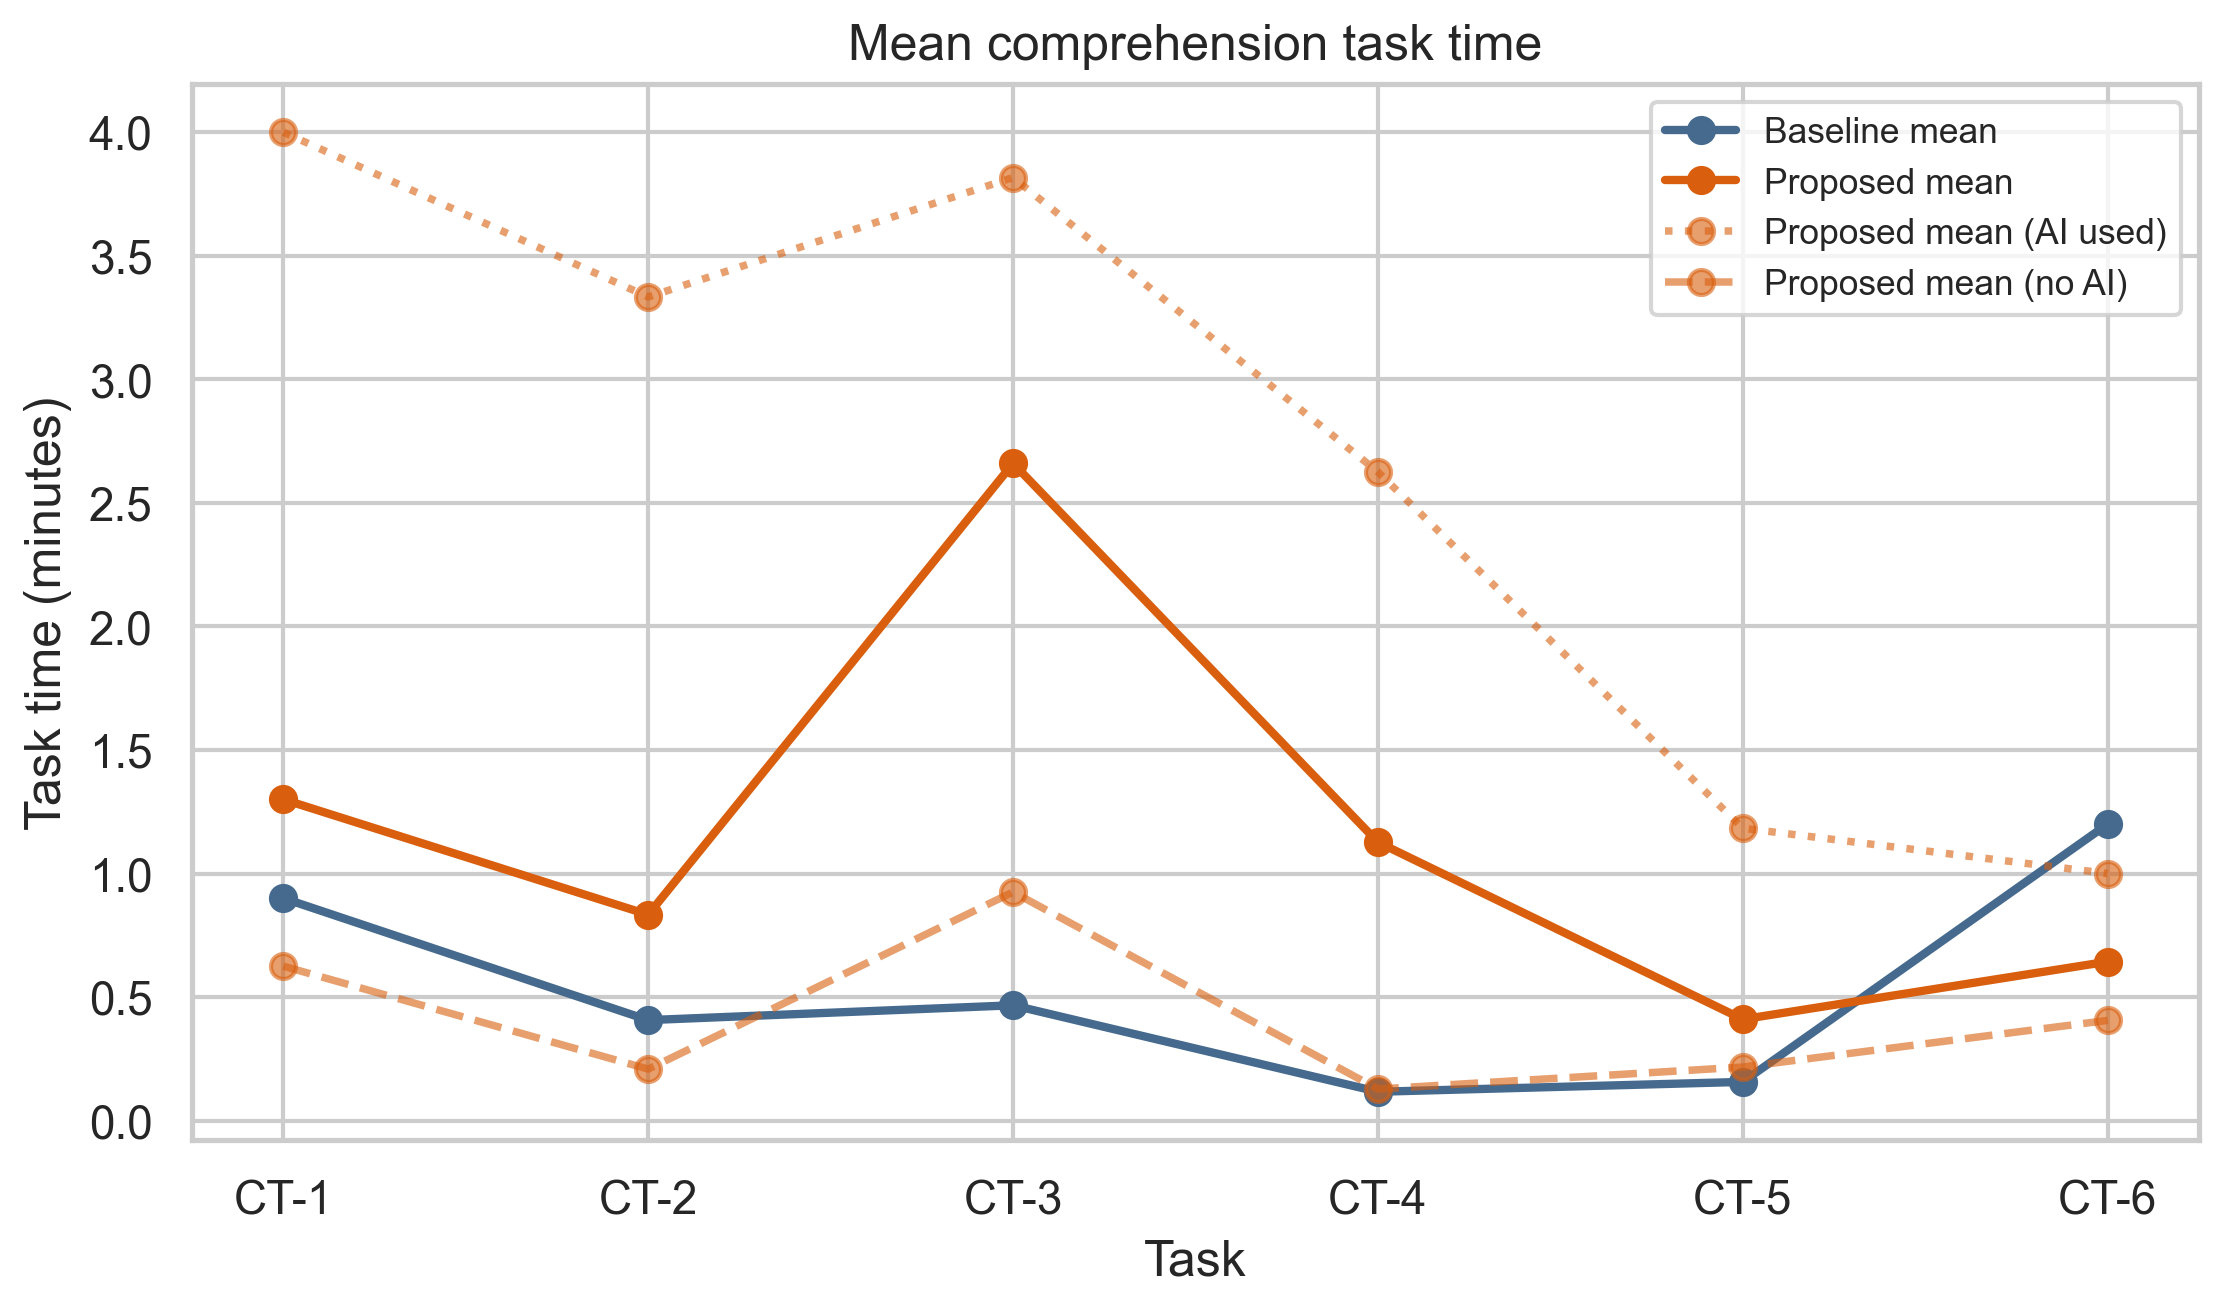
\includegraphics[width=0.88\columnwidth]{media/evaluation/time_by_task_order_with_ai_use_comprehension.png}
    \caption{Mean comprehension task (CT) time by task (CT-1--CT-6), comparing baseline (A) and proposed (B), with condition B split by whether the assistant was used on the task.}
    \label{fig:evaluation:time-by-task-ai-comp}
\end{figure}

% Figure \ref{fig:evaluation:time-participant-comp} shows the comprehension time by tasks for each participant (baseline dashed, proposed solid).

% \begin{figure}[H]
%     \centering
%     \includegraphics[width=0.88\columnwidth]{media/evaluation/task_time_per_participant_comprehension.png}
%     \caption{Comprehension task time by participant across tasks (baseline dashed, proposed solid).}
%     \label{fig:evaluation:time-participant-comp}
% \end{figure}

\subsubsection*{RQ3: How does the proposed system influence the correctness of modification and reuse of robot programs?}
The proposed system reduced modification correctness substantially relative to the baseline. In baseline, completed-only correctness was 1.00 (24/24), with DNF-inclusive correctness of 0.96 (24/25). In the proposed condition, completed-only correctness was 0.60 (12.5/21), and DNF-inclusive correctness was 0.50 (12.5/25). At the aggregate level, this is a substantial regression.

The aggregate, however, obscures considerable variation across modification task types. The five modification tasks behaved very differently. MT-2 (movement type change) remained perfect in both conditions (1.00 vs. 1.00). MT-3 (waypoint switch) showed a smaller decrease (1.00 vs. 0.80). In contrast, MT-1 (speed modification) dropped to 0.20, MT-4 (blend enablement) to 0.50, every participant scored partial credit, the full mark required also specifying the blend radius, which no participant did. MT-5 (wait node addition) dropped to 0.00.

This pattern points to a structural failure rather than a general inability to modify programs with the proposed system. Participants performed relatively well when updating existing values (MT-2 and MT-3), but struggled on tasks requiring parameter disambiguation (MT-1) and node insertion (MT-4 and MT-5) in the raw \texttt{.urpx} structure.

\subsubsection*{RQ4: How does the proposed system influence the time required in the modification and reuse of robot programs?}
The proposed system also increased modification time substantially. Mean modification time per participant increased from 4.85 to 9.81 minutes, and the median increased from 4.03 to 12.53 minutes. The paired Wilcoxon test gave $p = 0.44$ ($n=5$), with a large effect size ($\delta = +0.52$). Completion rate also dropped (0.96 baseline vs. 0.84 proposed). As for comprehension, the Wilcoxon result is not statistically significant with $n=5$, but Cliff's delta indicates a large directional effect toward longer modification times in the proposed condition.

Unlike comprehension, this penalty remained large after subtracting assistant wait time. Mean active modification time in the proposed condition was 8.04 minutes, and the active-time effect size remained $\delta = +0.52$. This indicates that modification work itself was slower in the proposed workflow, not only delayed by assistant latency.

The task-level breakdown in Figure \ref{fig:evaluation:time-by-task-ai-mod} shows the same pattern when the proposed mean is split by assistant use. The proposed \textit{without-assistant} means were close to baseline for MT-1, MT-2, and MT-4 (MT-1: $+5.7$ s, MT-2: $+3.6$ s, MT-4: $+4.6$ s), while MT-3 was faster than baseline ($-187.0$ s). In contrast, the proposed \textit{with-assistant} means were higher than baseline across all modification tasks (MT-1: $+246.9$ s, MT-2: $+34.6$ s, MT-3: $+130.8$ s, MT-4: $+164.6$ s, MT-5: $+82.4$ s). For MT-5, all completed proposed-condition attempts used the assistant, so there is no corresponding without-assistant mean.

Assistant logs for modification tasks indicate a heavier latency profile than in comprehension. Across 19 modification-linked sessions, mean response time was 55.57 s (median 46.19 s). Mean embedding time was 4.12 s per call. The 5-call retrieval cap was reached in 26.3\% of modification sessions (5/19), and those capped sessions averaged 82.07 s. This is consistent with the larger remaining modification-time penalty, where assistant-related delay is more prominent and more variable.

\begin{figure}[H]
    \centering
    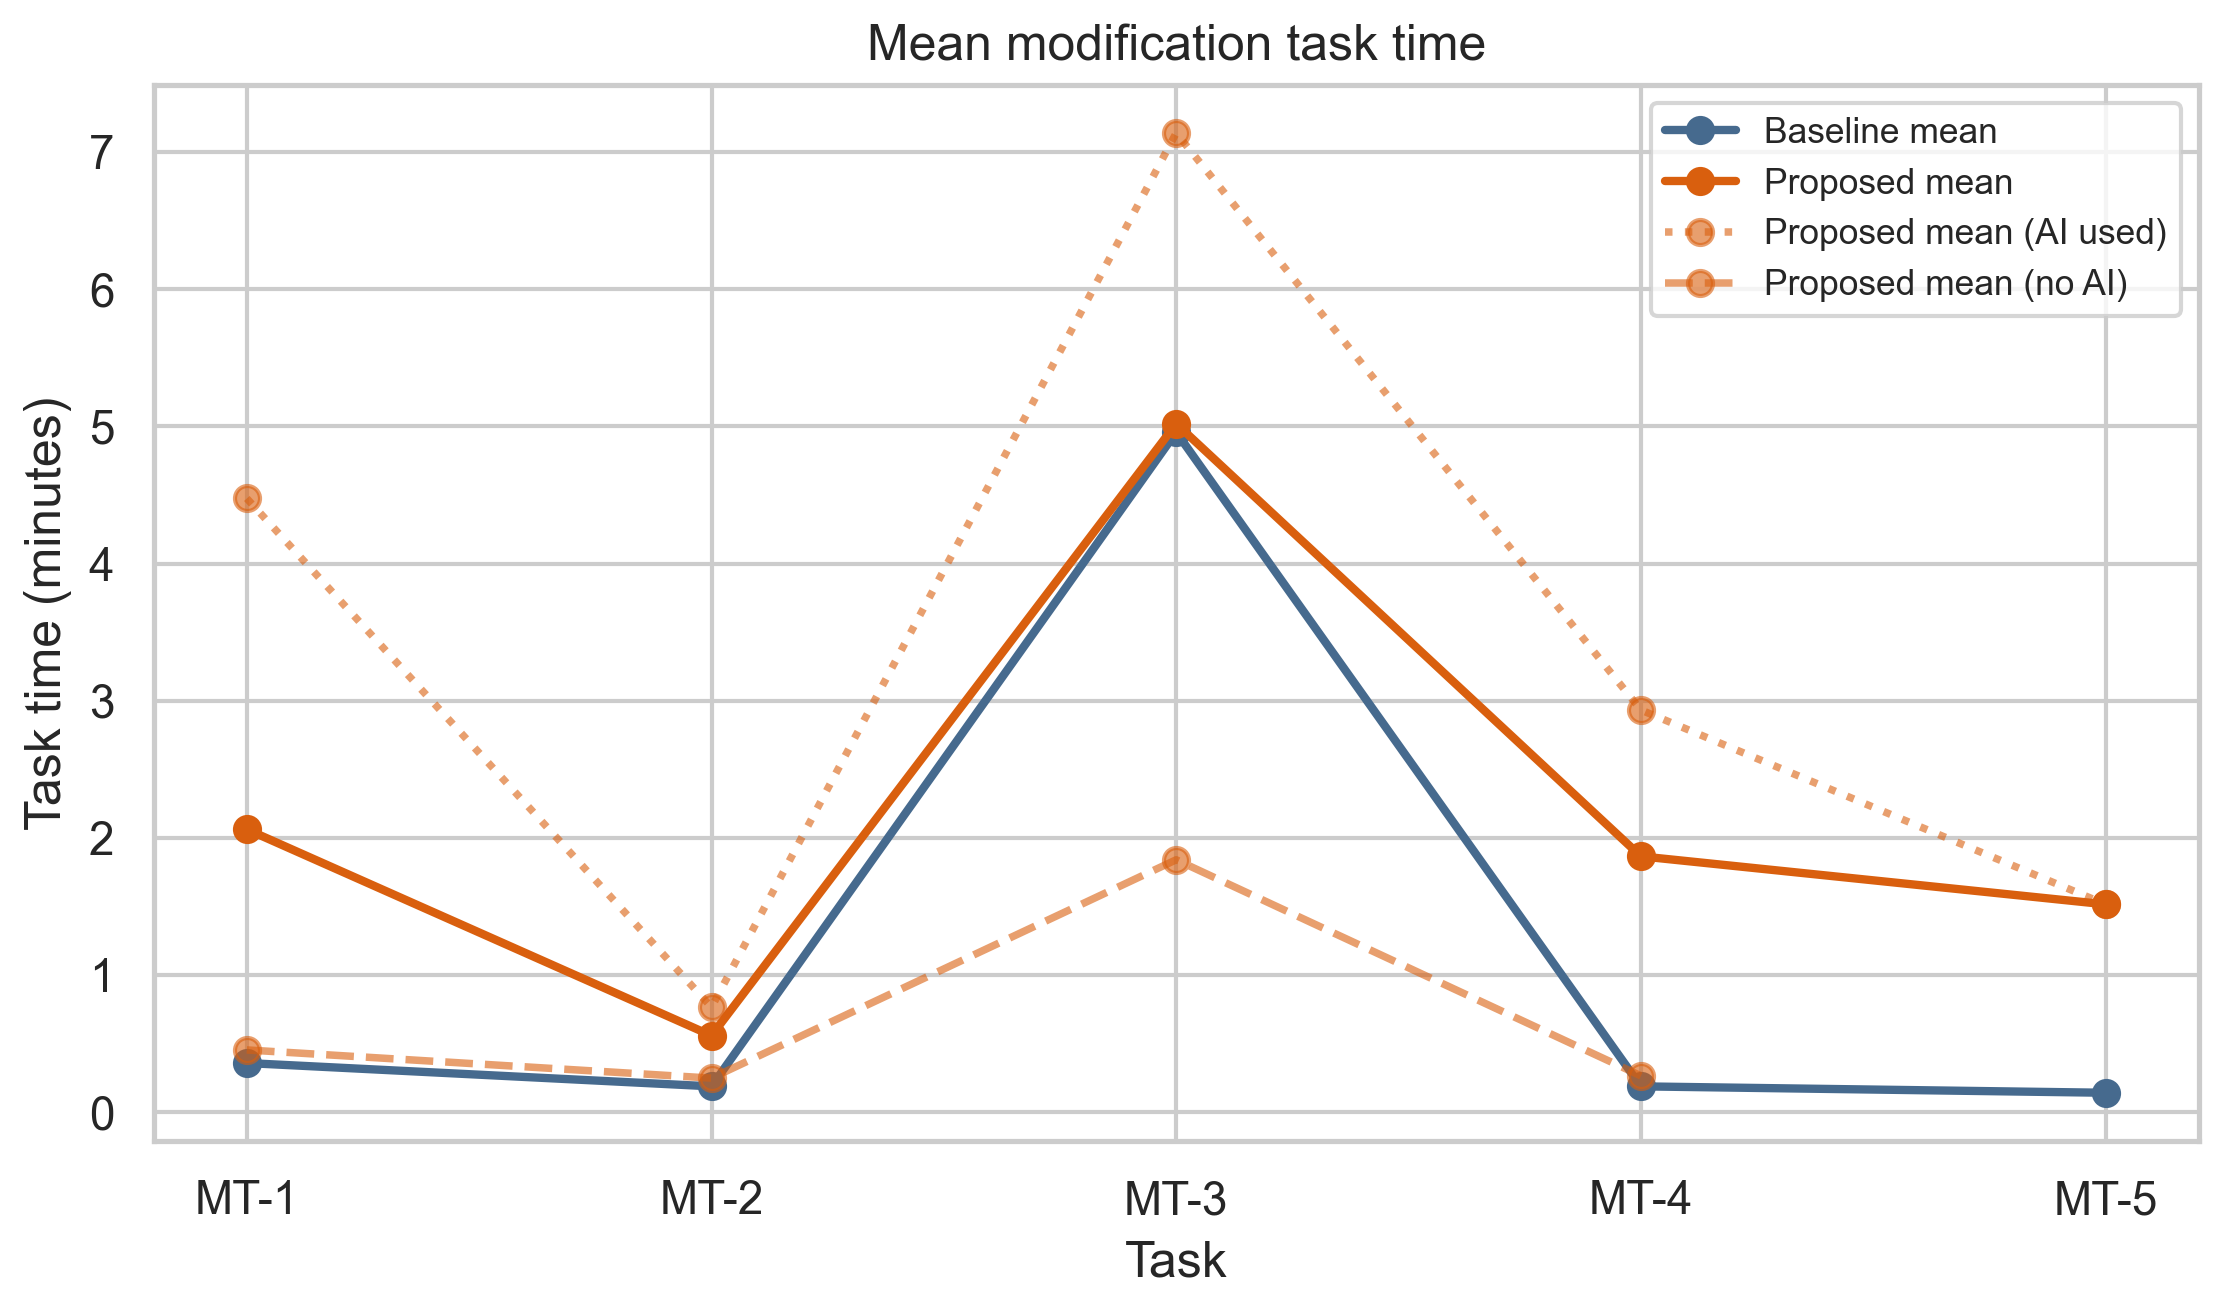
\includegraphics[width=0.88\columnwidth]{media/evaluation/time_by_task_order_with_ai_use_modification.png}
    \caption{Mean modification task (MT) time by task (MT-1 -- MT-5), comparing baseline (A) and proposed (B), with condition B split by whether the assistant was used on the task.}
    \label{fig:evaluation:time-by-task-ai-mod}
\end{figure}

% \begin{figure}[H]
%     \centering
%     \includegraphics[width=0.88\columnwidth]{media/evaluation/task_time_per_participant_modification.png}
%     \caption{Modification task (MT-1--MT-5) time by participant (baseline dashed, proposed solid).}
%     \label{fig:evaluation:time-participant-mod}
% \end{figure}

\subsubsection*{Confidence}
Self-reported confidence was lower with the proposed system than with baseline for both comprehension (2.00 vs. 4.40) and modification (2.60 vs. 3.40), as shown in Figure \ref{fig:evaluation:confidence}.

Notably, there is a comprehension-confidence gap. Participants reported very low confidence in the proposed condition (2.00), even though comprehension correctness remained high (0.97, with only one incorrect response across all comprehension answers). This suggests that participants were often unsure about their answers while working in the raw \texttt{.urpx} representation, even when they ultimately answered correctly. In contrast, modification shows both lower confidence and substantially lower correctness, indicating that participants' lower confidence in modification more closely reflected actual difficulties.

\begin{figure}[H]
    \centering
    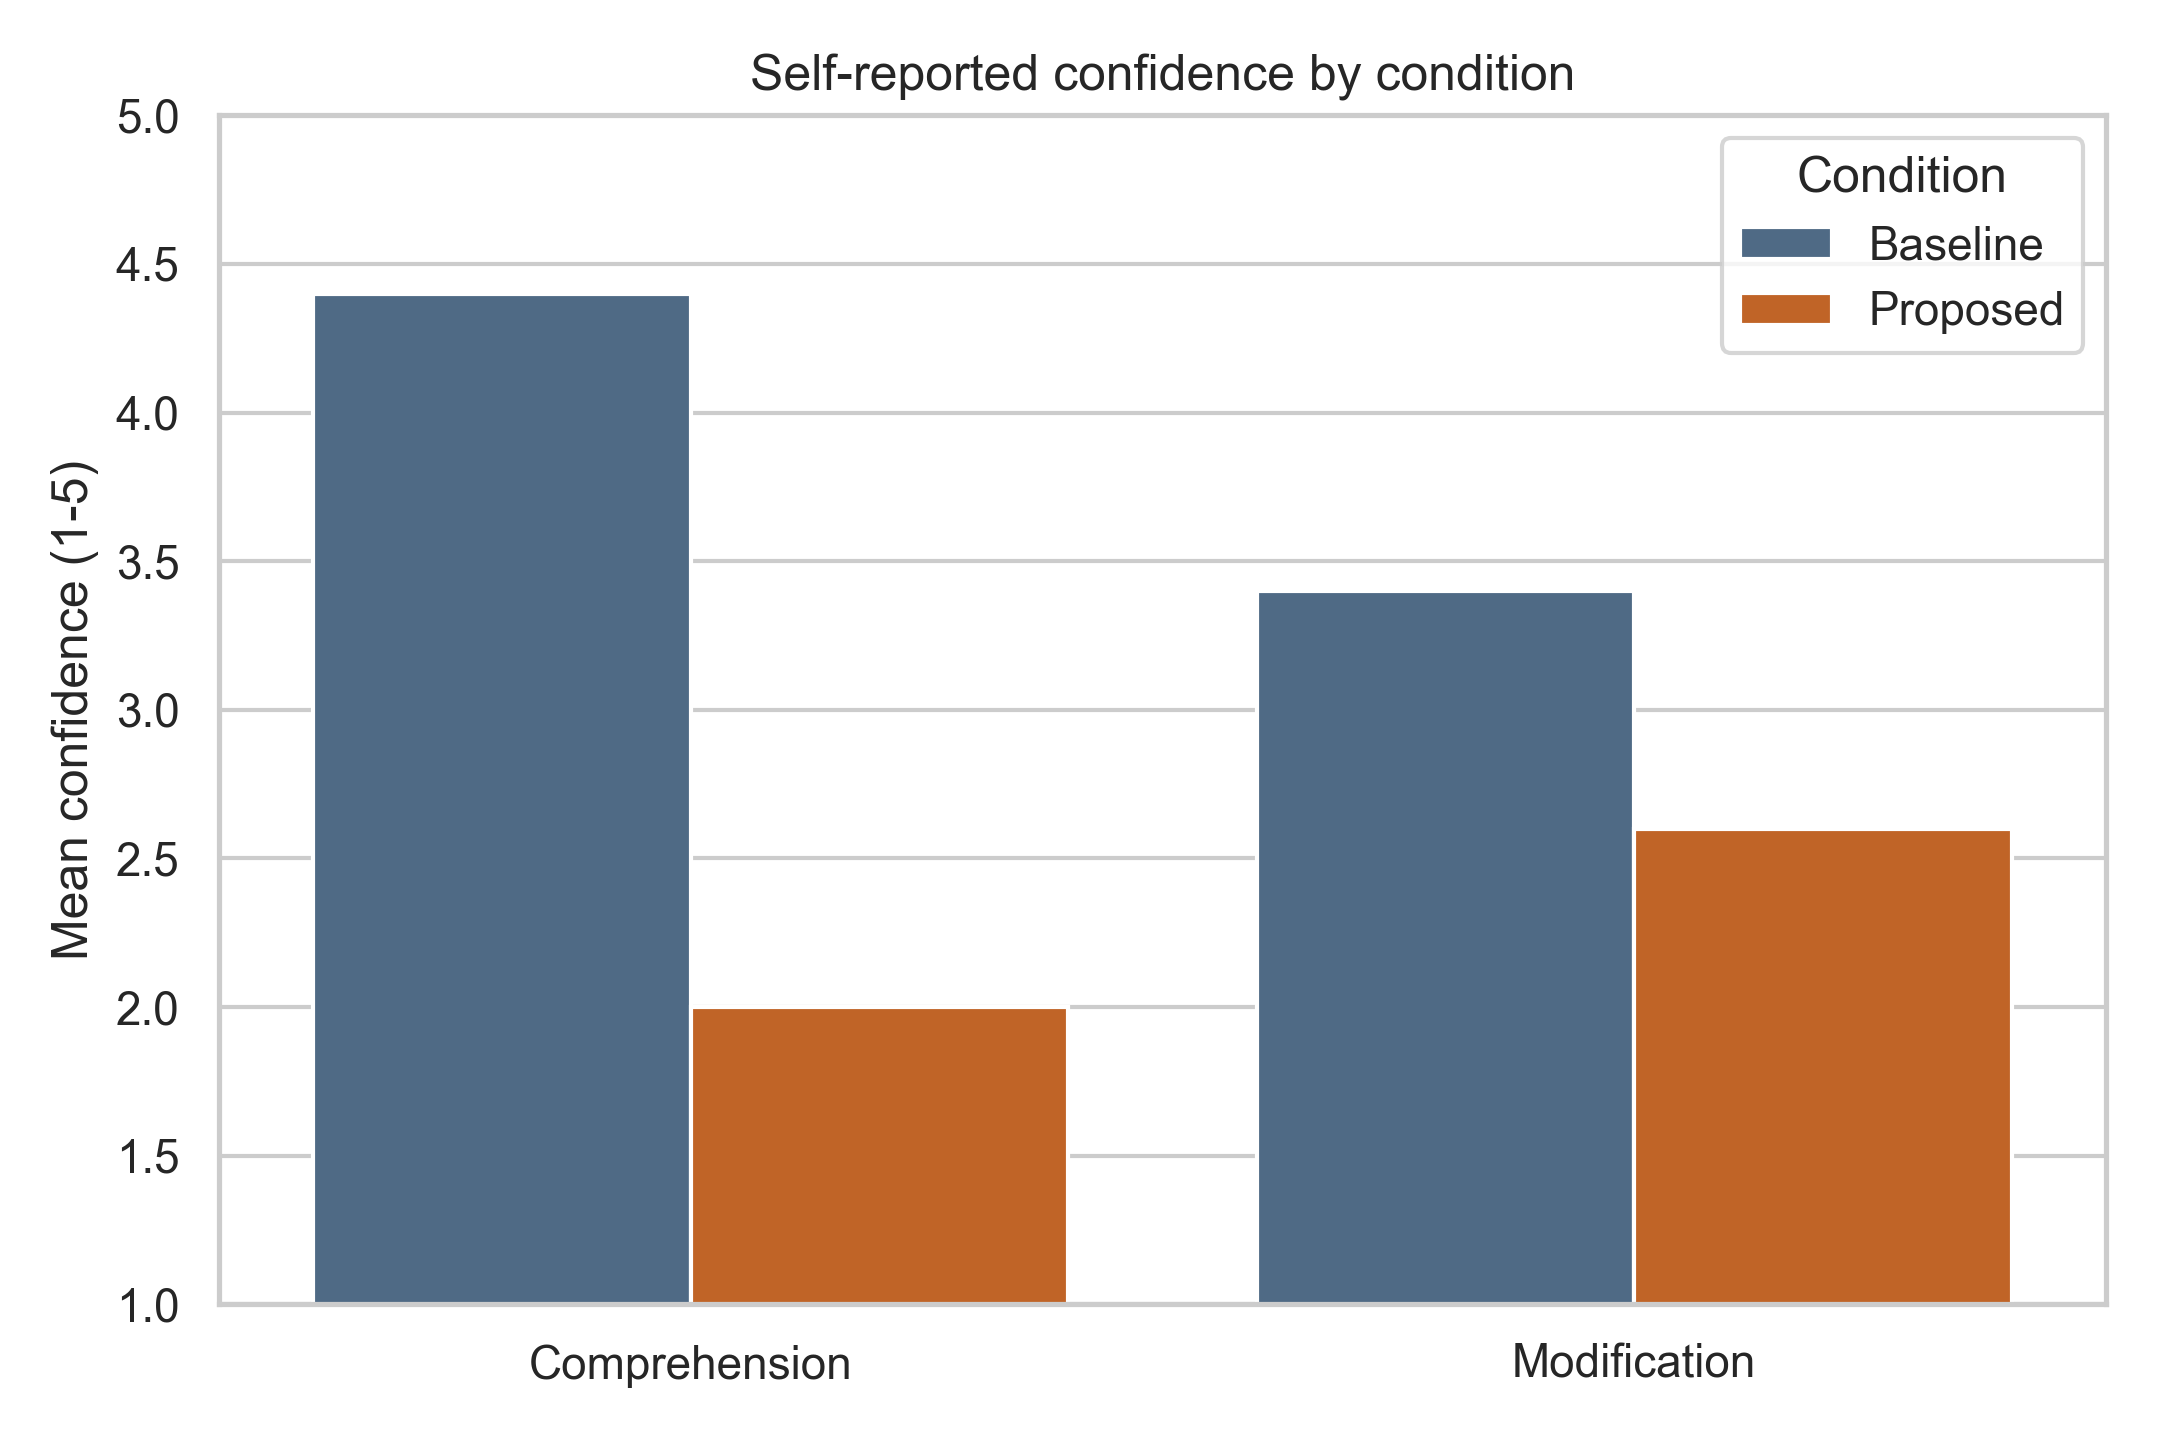
\includegraphics[width=0.62\columnwidth]{media/evaluation/confidence_by_condition.png}
    \caption{Mean self-reported confidence (Likert 1-5) for comprehension and modification by condition.}
    \label{fig:evaluation:confidence}
\end{figure}


\subsubsection*{AI Assistant Usage and Latency}
The AI assistant was used in 26 of 55 possible task opportunities in condition B (47.3\%). Usage varied by task and was highest for MT-5 (100\% of participants). The next-highest usage was 60\% on CT-3, MT-2, MT-3, and MT-4. Figure \ref{fig:evaluation:ai-usage} shows assistant usage rates per task.

\begin{figure}[H]
    \centering
    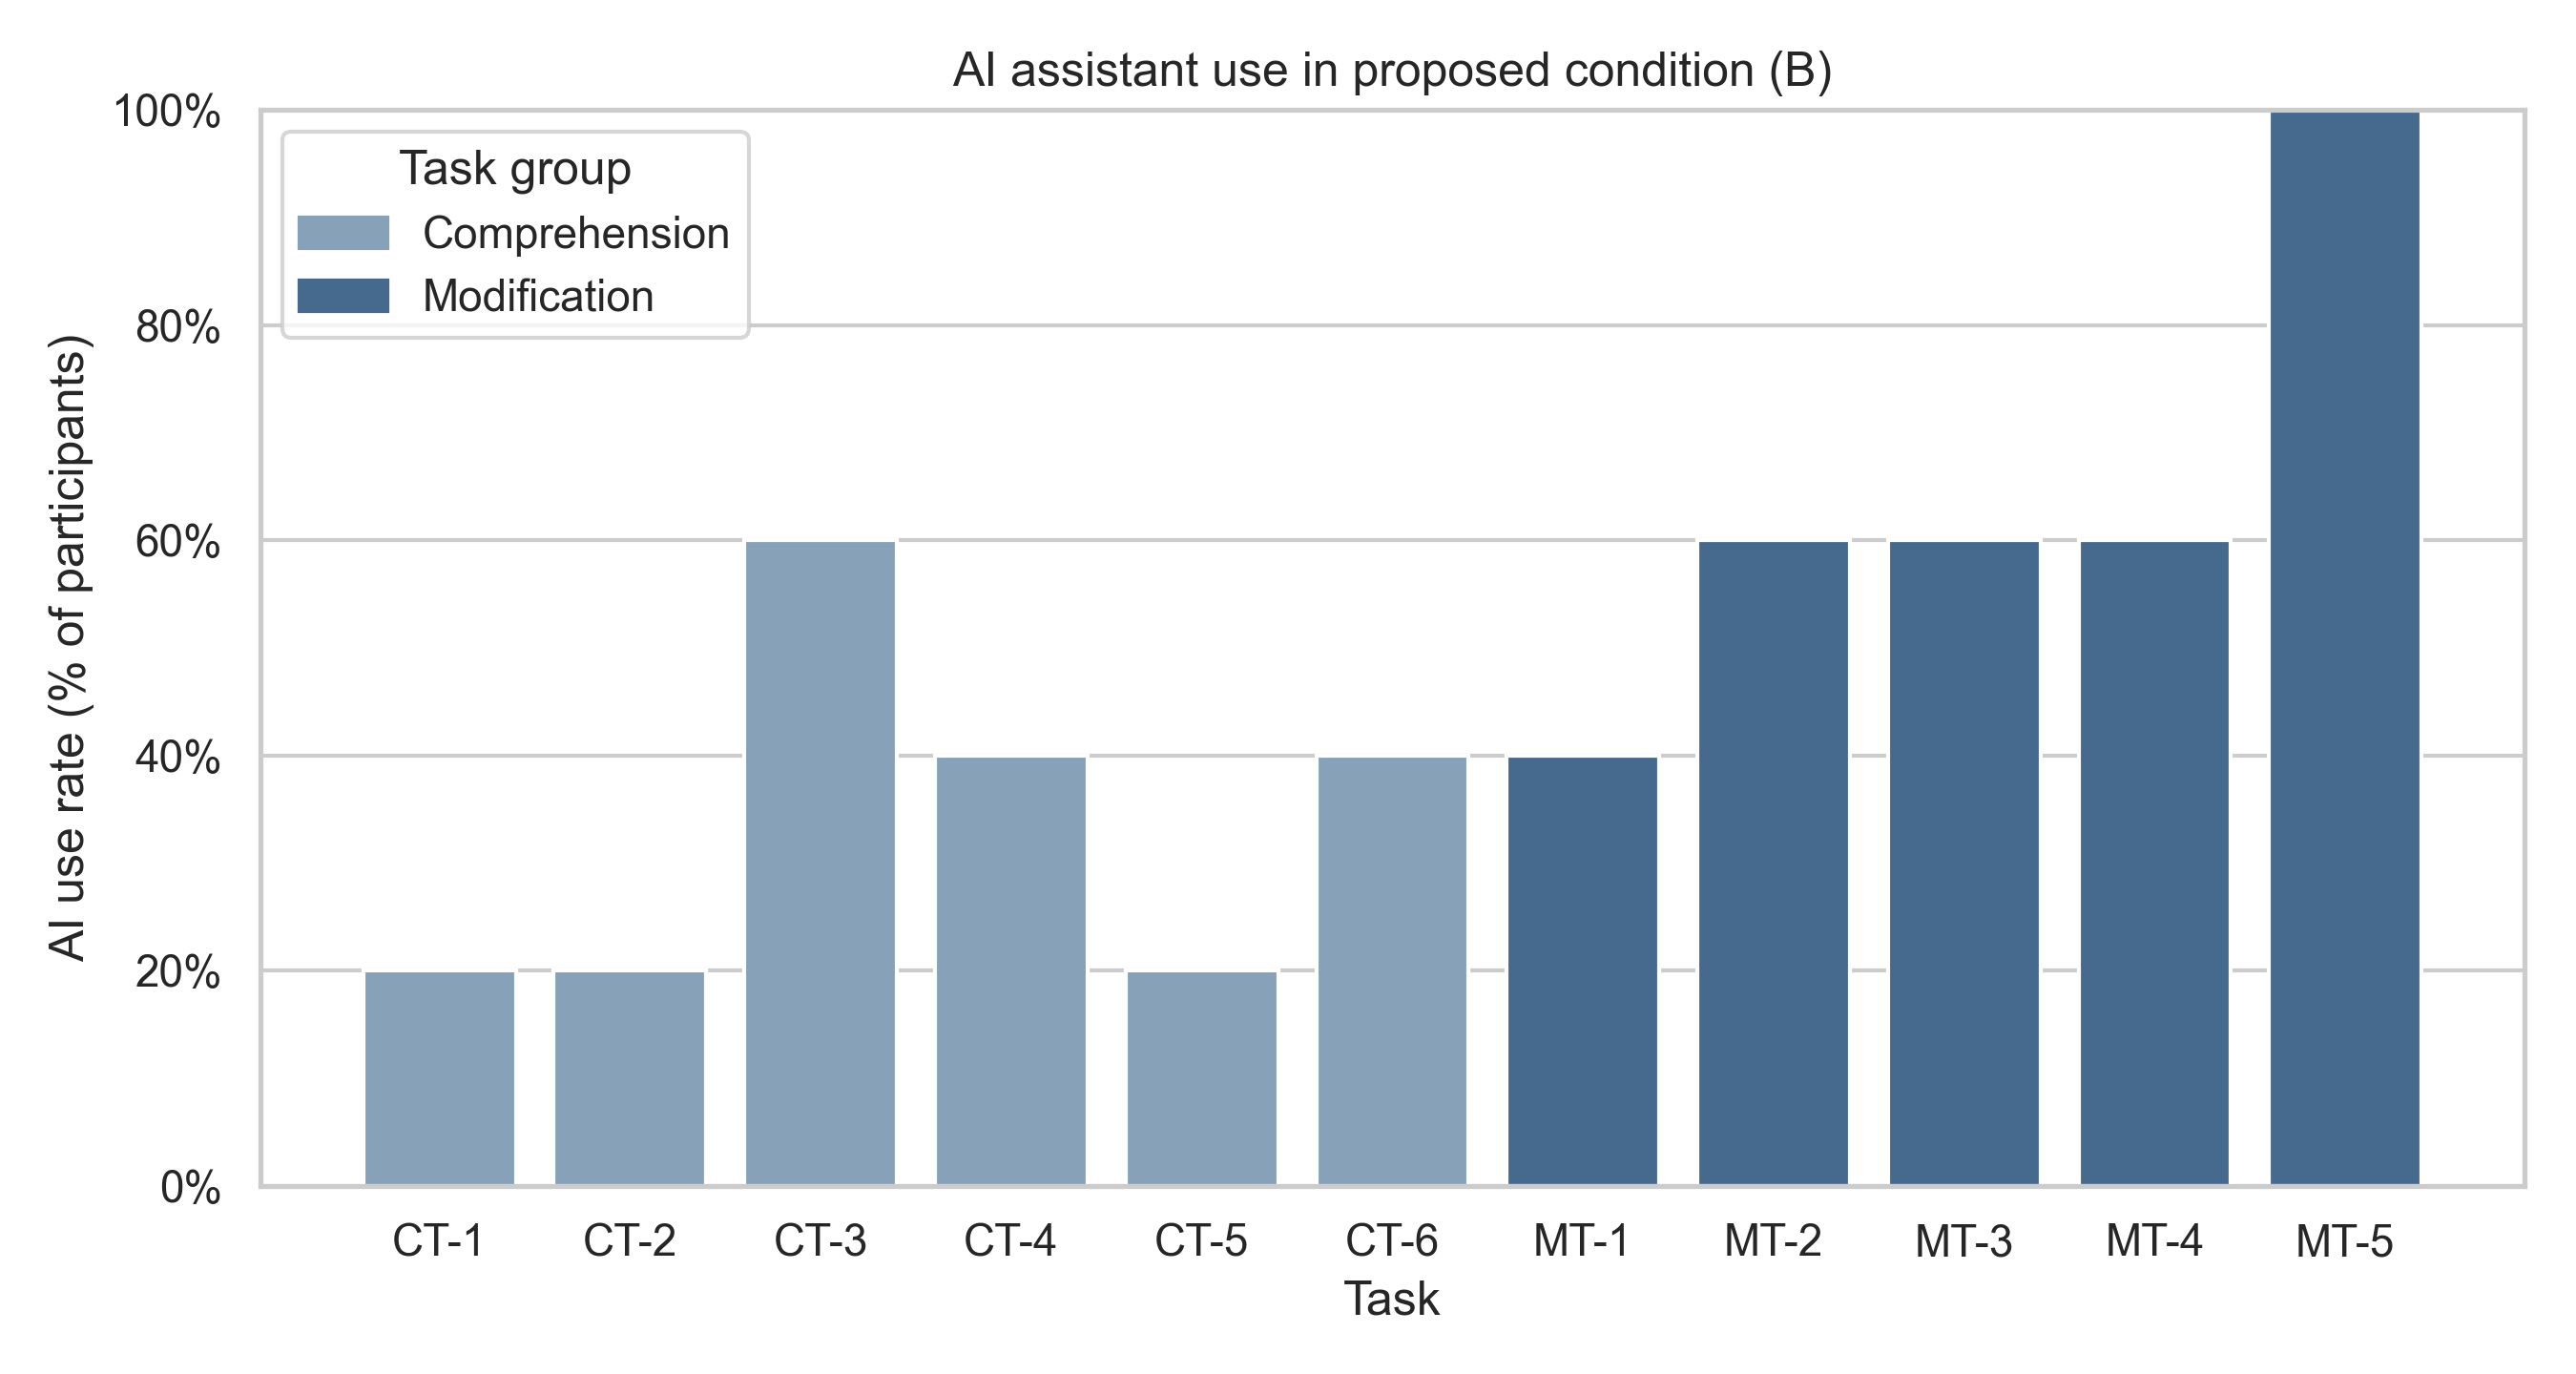
\includegraphics[width=0.82\columnwidth]{media/evaluation/ai_use_rate_by_task.png}
    \caption{AI assistant usage rate by task in condition B (CT-1 -- CT-6 and MT-1 -- MT-5).}
    \label{fig:evaluation:ai-usage}
\end{figure}

Figure \ref{fig:evaluation:assistant-latency-tools} shows the relationship between assistant response time and number of tool calls per assistant request. Across all 43 assistant requests, mean response time was 47.41 s (median 42.56 s). Latency increased with tool-call count. Queries that included program context were slower on average than queries without program context (49.64 s vs. 41.64 s), as reflected by the color split in the plot.

This plot should be interpreted with two caveats. First, the analysis does not explicitly model conversation history or assistant memory carry-over across consecutive sessions. This may partly explain the \textit{no-context} outlier and some of the increasing variability at higher tool-call counts: more retrieved content and prior context can increase effective context-window load. Second, the current context flag is binary and does not distinguish context amount (e.g., a single node snippet vs. an entire program). Thus, the observed latency difference between context and no-context queries may be influenced by the amount of context included in the query, rather than the presence of context alone.

\begin{figure}[H]
    \centering
    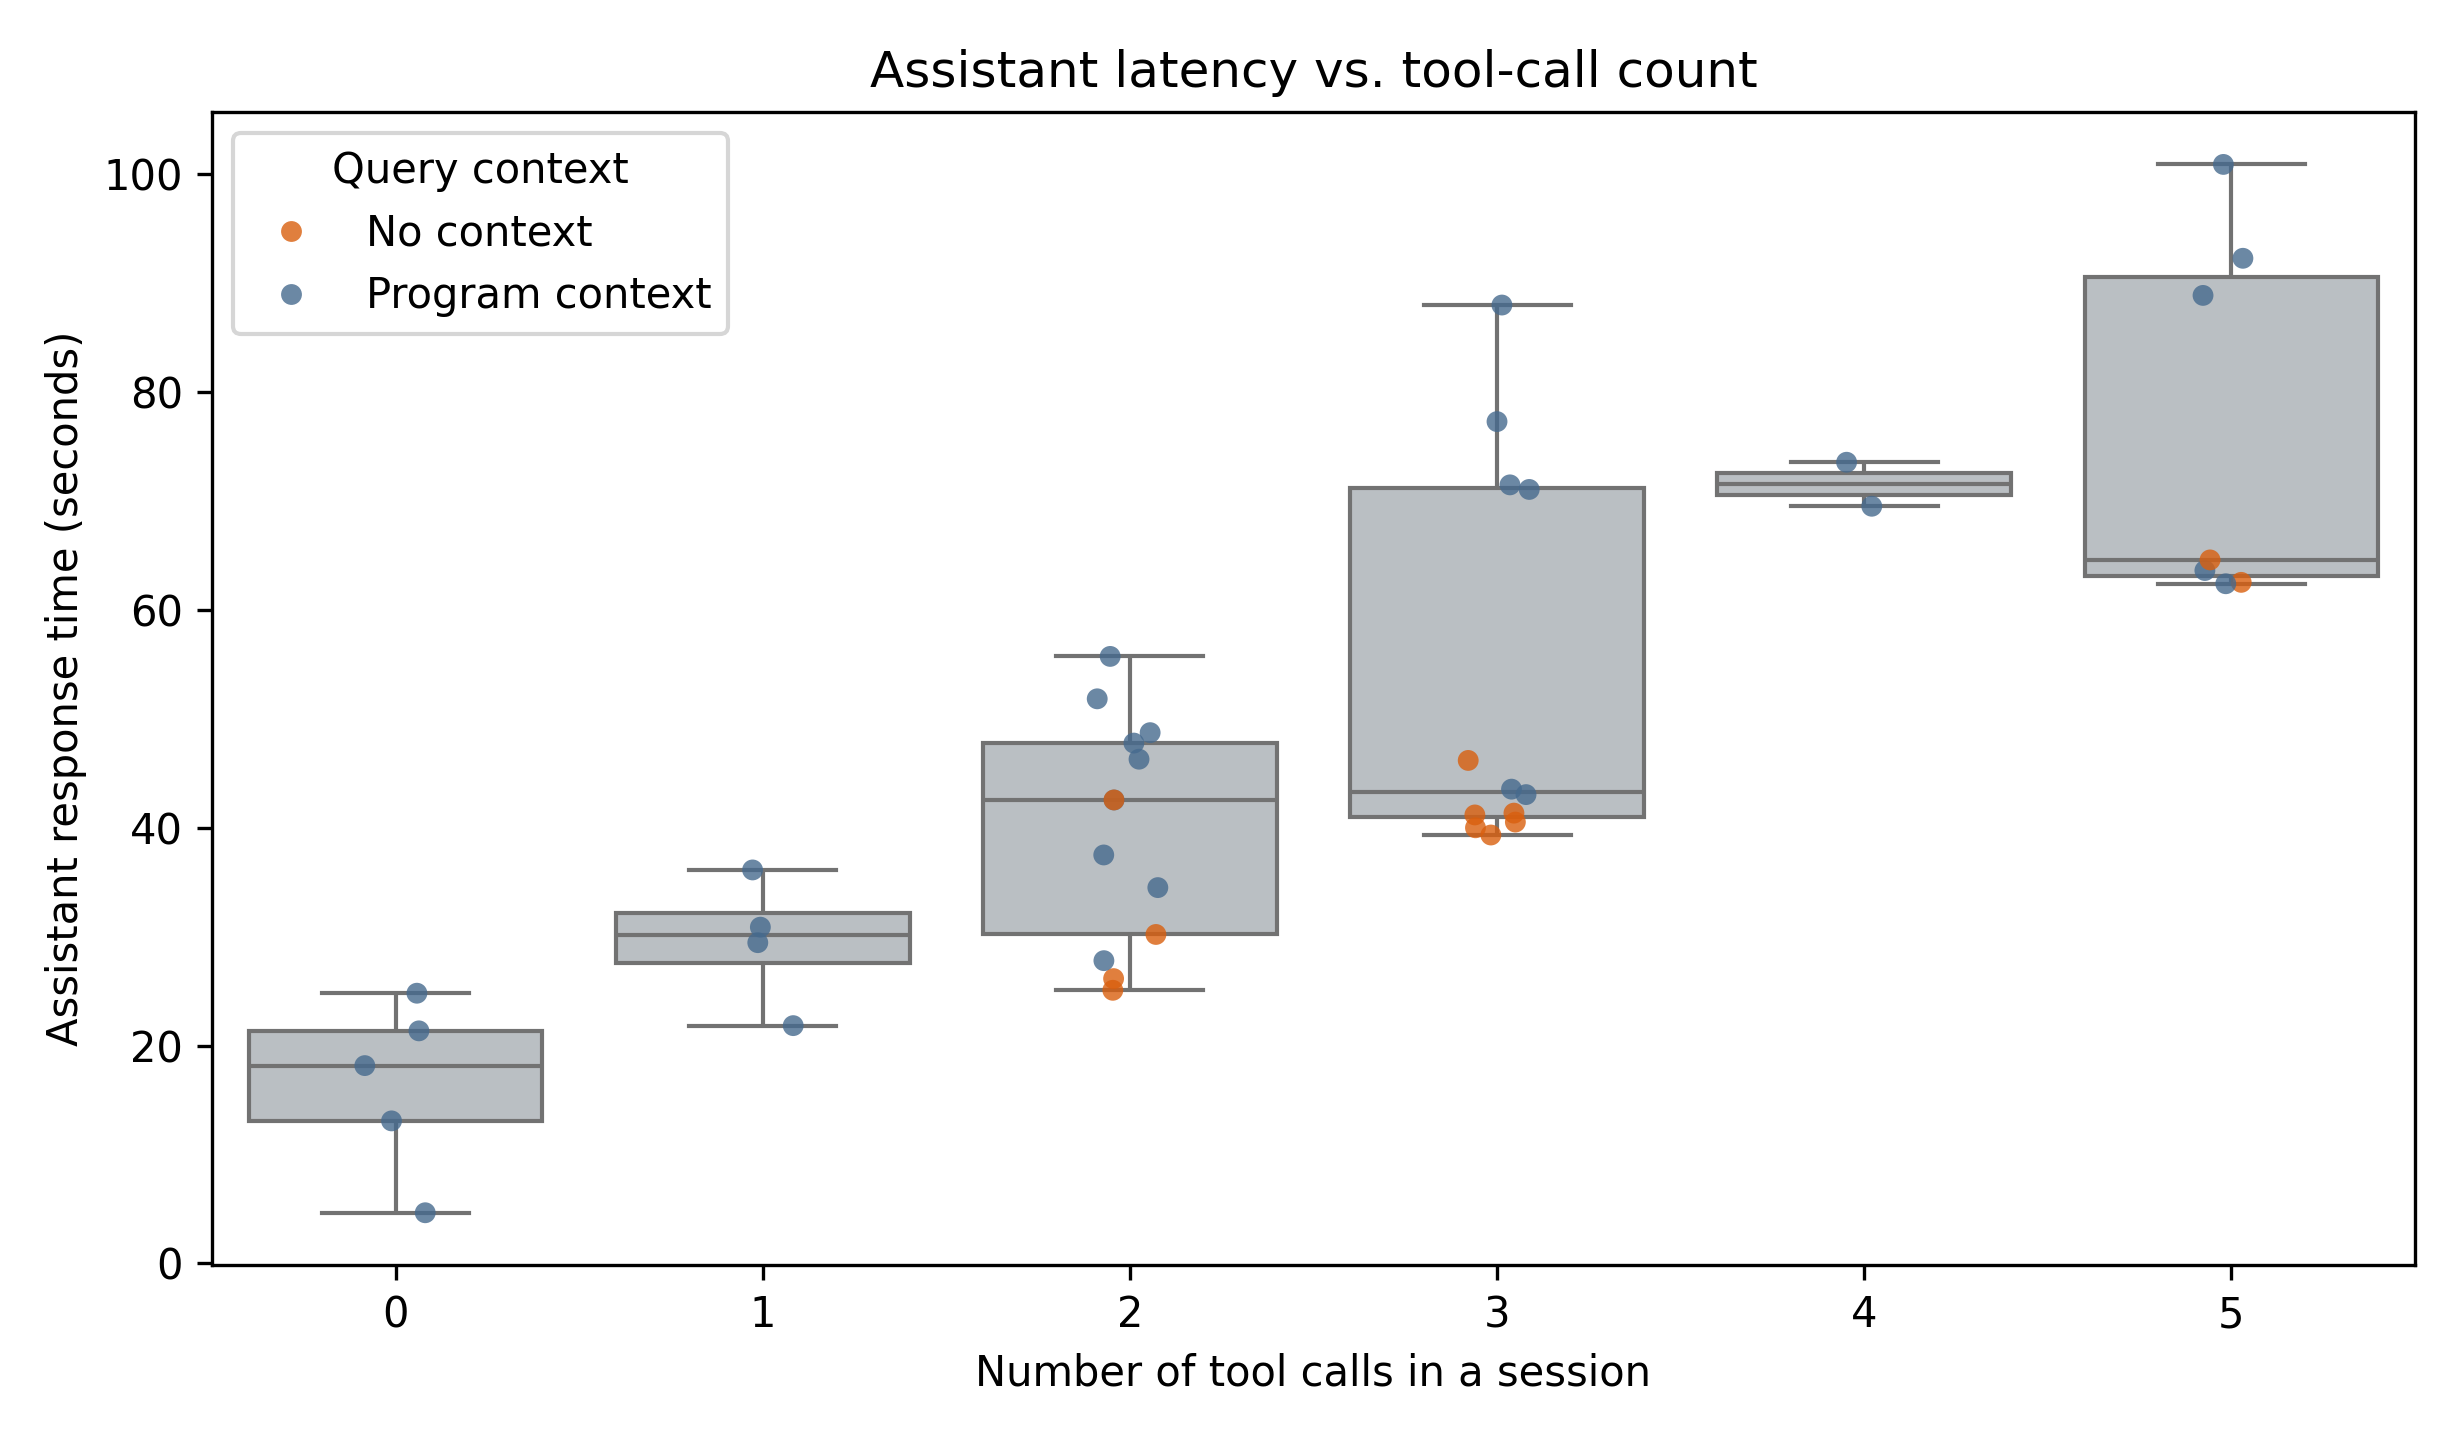
\includegraphics[width=0.82\columnwidth]{media/evaluation/assistant_latency_by_tool_calls.png}
    \caption{AI assistant response time by number of tool calls per assistant request. Points are colored by whether the user included program context in the query.}
    \label{fig:evaluation:assistant-latency-tools}
\end{figure}


\subsection{Post-Study Questionnaire}
Participants provided post-study ratings on various aspects of the system and their experience. The following sections summarize the key findings from these ratings.

\paragraph{Response Comprehension}~\\
The comprehension-response ratings indicate a mixed pattern (Figure \ref{fig:evaluation:post-study-response-comprehension}). Clarity was rated positively by all participants, suggesting that the assistant output was generally readable and understandable. In contrast, ratings for relevance and factual correctness were mostly negative, and quality ratings were split between positive, neutral, and negative responses. Overall, participants could often understand the responses, but frequently questioned whether the content was correct and well aligned with their query.

\begin{figure}[H]
    \centering
    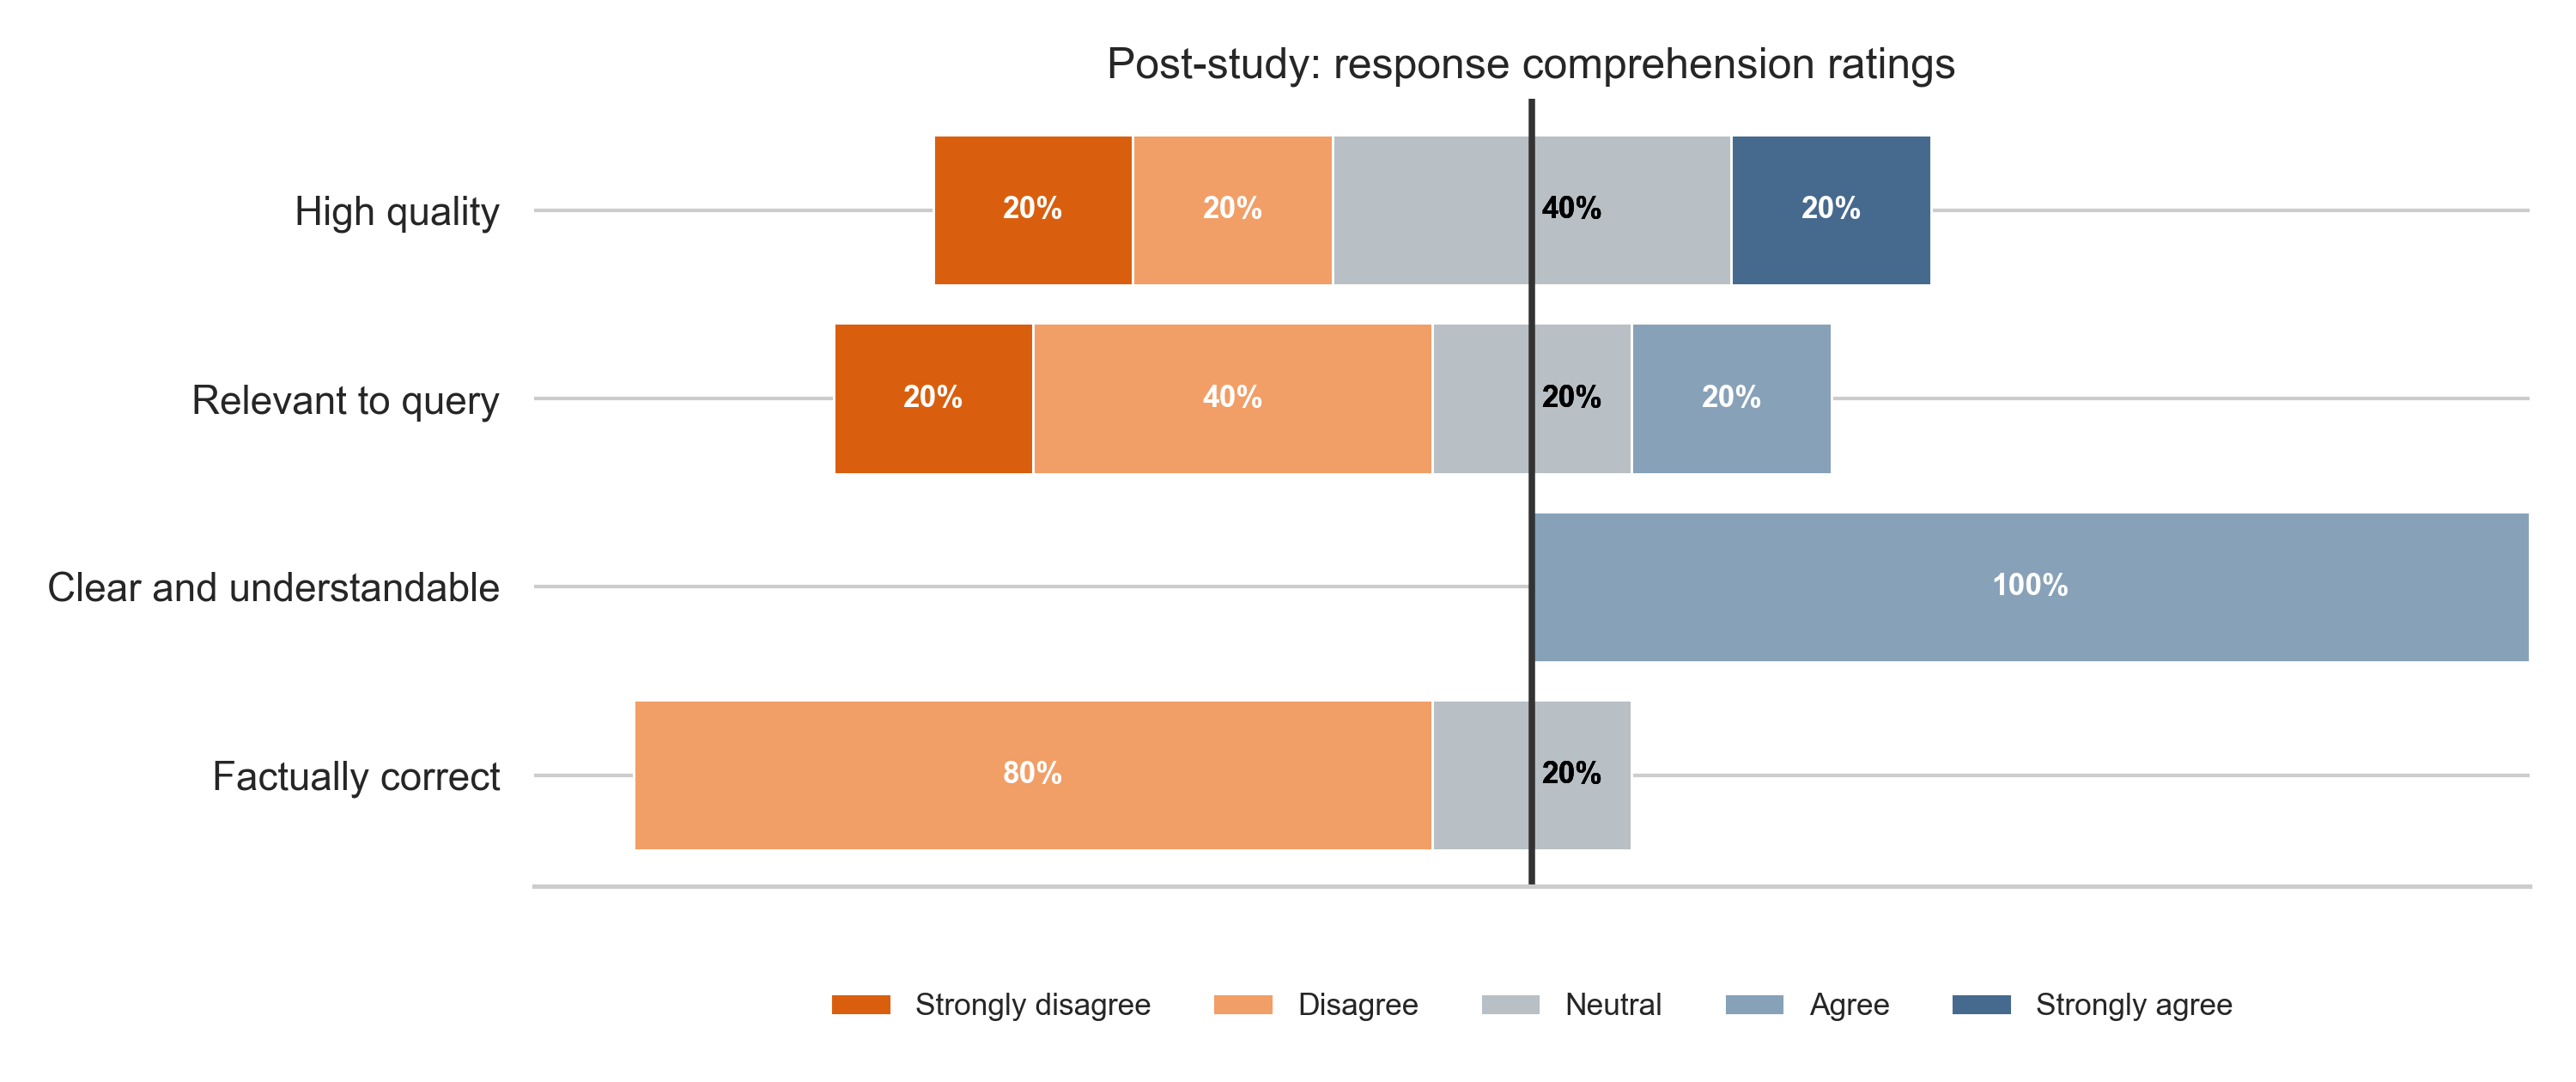
\includegraphics[width=\columnwidth]{media/evaluation/post_study_response_comprehension_diverging.png}
    \caption{Post-study ratings of assistant comprehension responses (quality, relevance, clarity, and factual correctness) shown as a divergent stacked Likert chart.}
    \label{fig:evaluation:post-study-response-comprehension}
\end{figure}

\paragraph{Response Modification}~\\
For modification-response ratings (Figure \ref{fig:evaluation:post-study-response-modification}), clarity again trended more positively than the other dimensions. However, quality and relevance were mainly neutral-to-negative, and factual correctness was rated mostly negatively. This indicates that even when suggestions were understandable, participants often did not consider them sufficiently accurate or directly usable for completing modification tasks.

\begin{figure}[H]
    \centering
    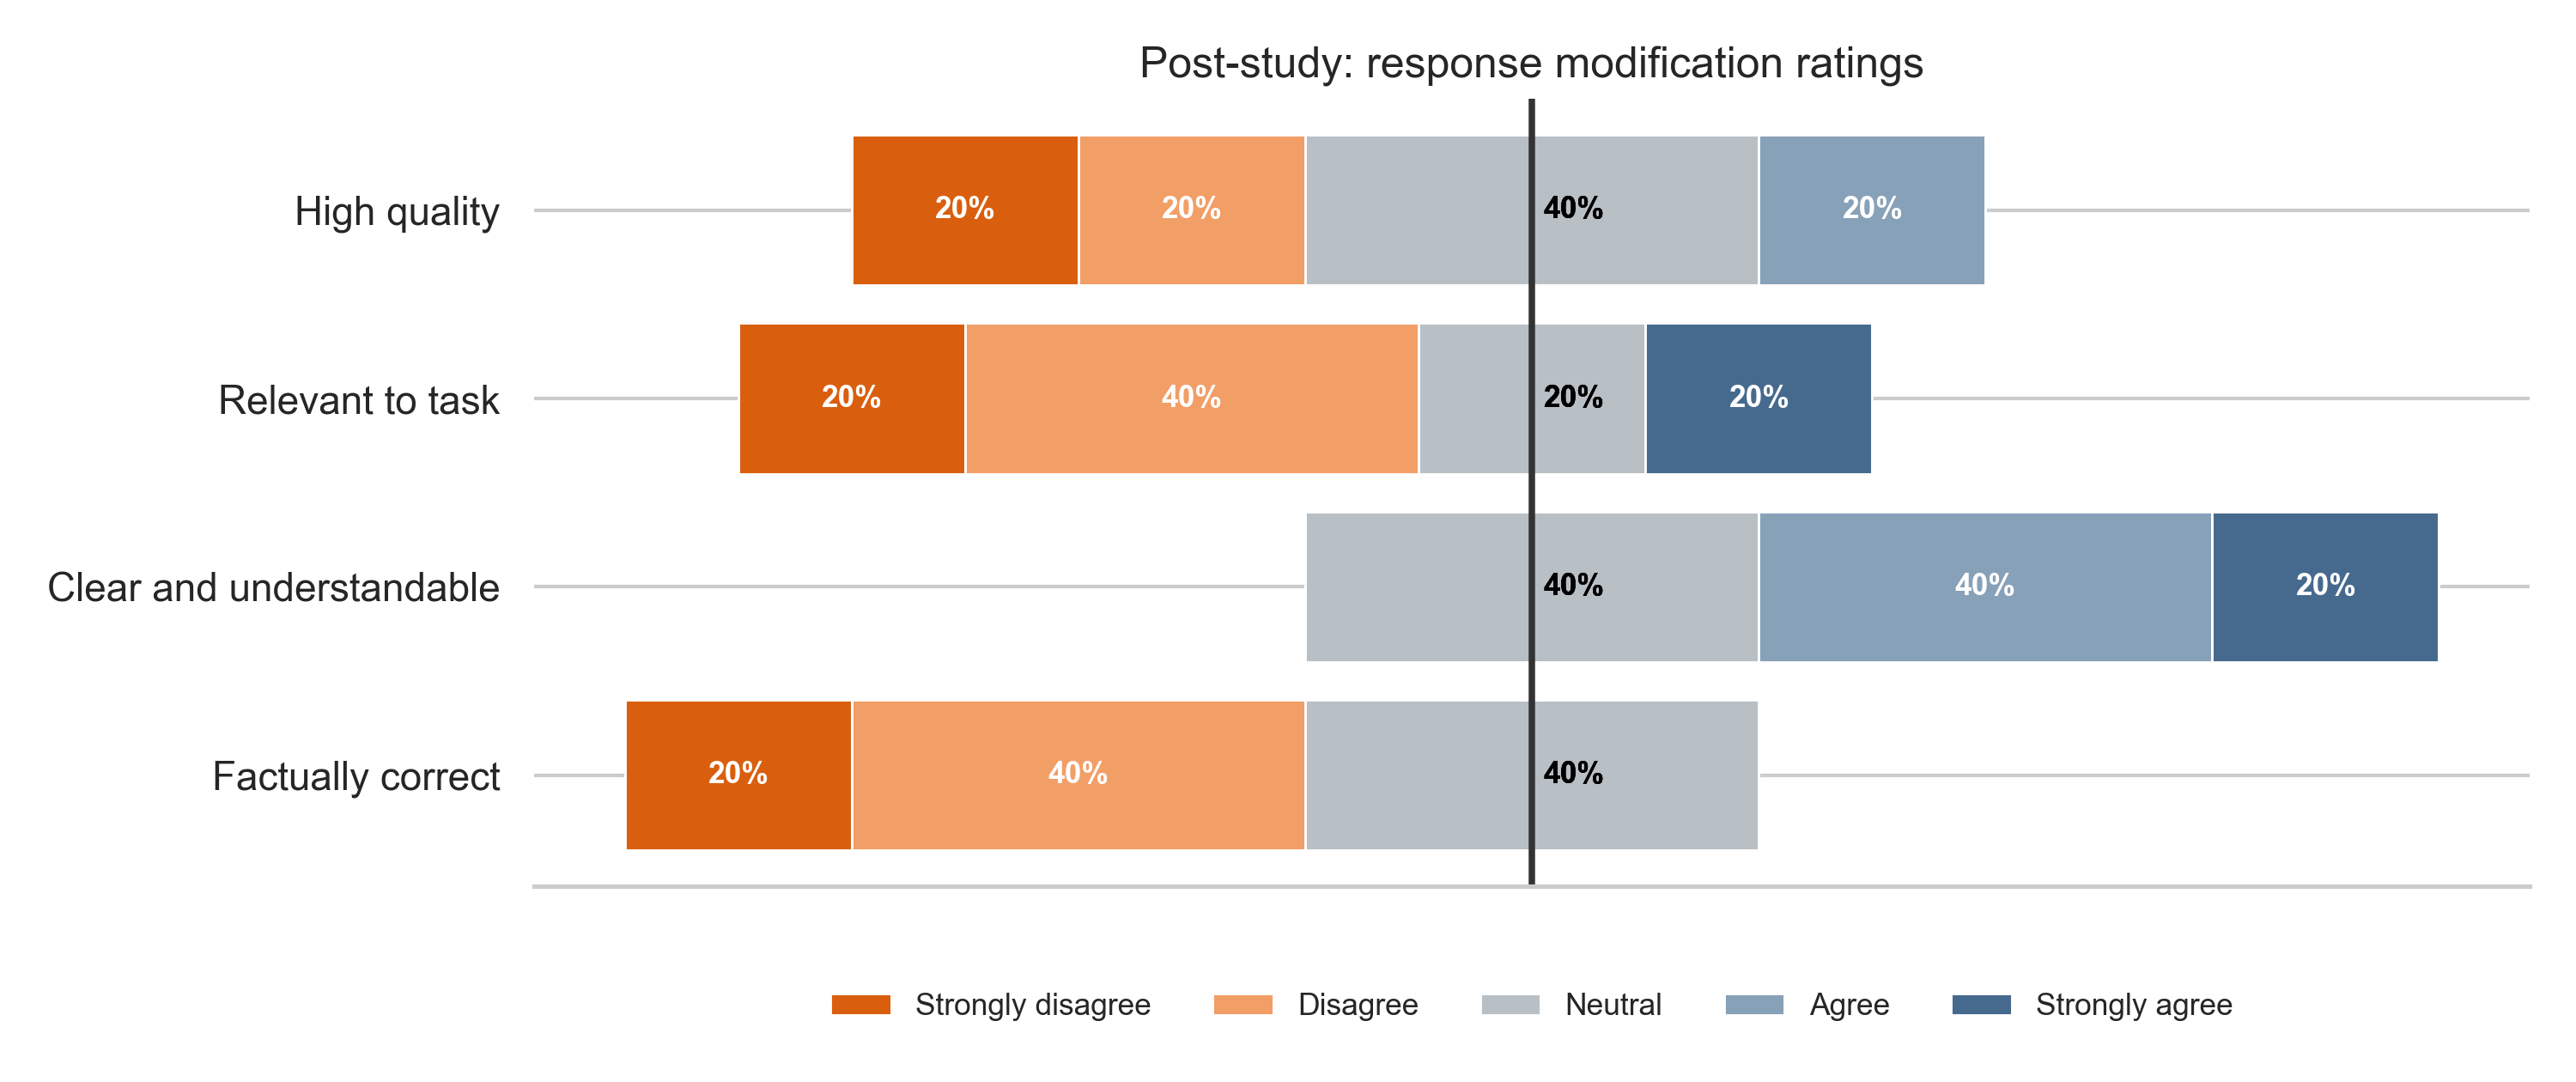
\includegraphics[width=\columnwidth]{media/evaluation/post_study_response_modification_diverging.png}
    \caption{Post-study ratings of assistant modification responses (quality, relevance, clarity, and factual correctness) shown as a divergent stacked Likert chart.}
    \label{fig:evaluation:post-study-response-modification}
\end{figure}

\paragraph{System Usability}~\\
System-usability ratings (Figure \ref{fig:evaluation:post-study-system-usability}) further reflect this tension. Ease of use was polarized, with both clearly positive and clearly negative ratings. Perceived usefulness for robotic program development was predominantly negative, and willingness to use the system in its current form was also mostly negative (with one strong positive outlier). This suggests that while some participants saw potential value in the system, most were not satisfied with its current performance and would not choose to use it for real work without significant improvements.

\begin{figure}[H]
    \centering
    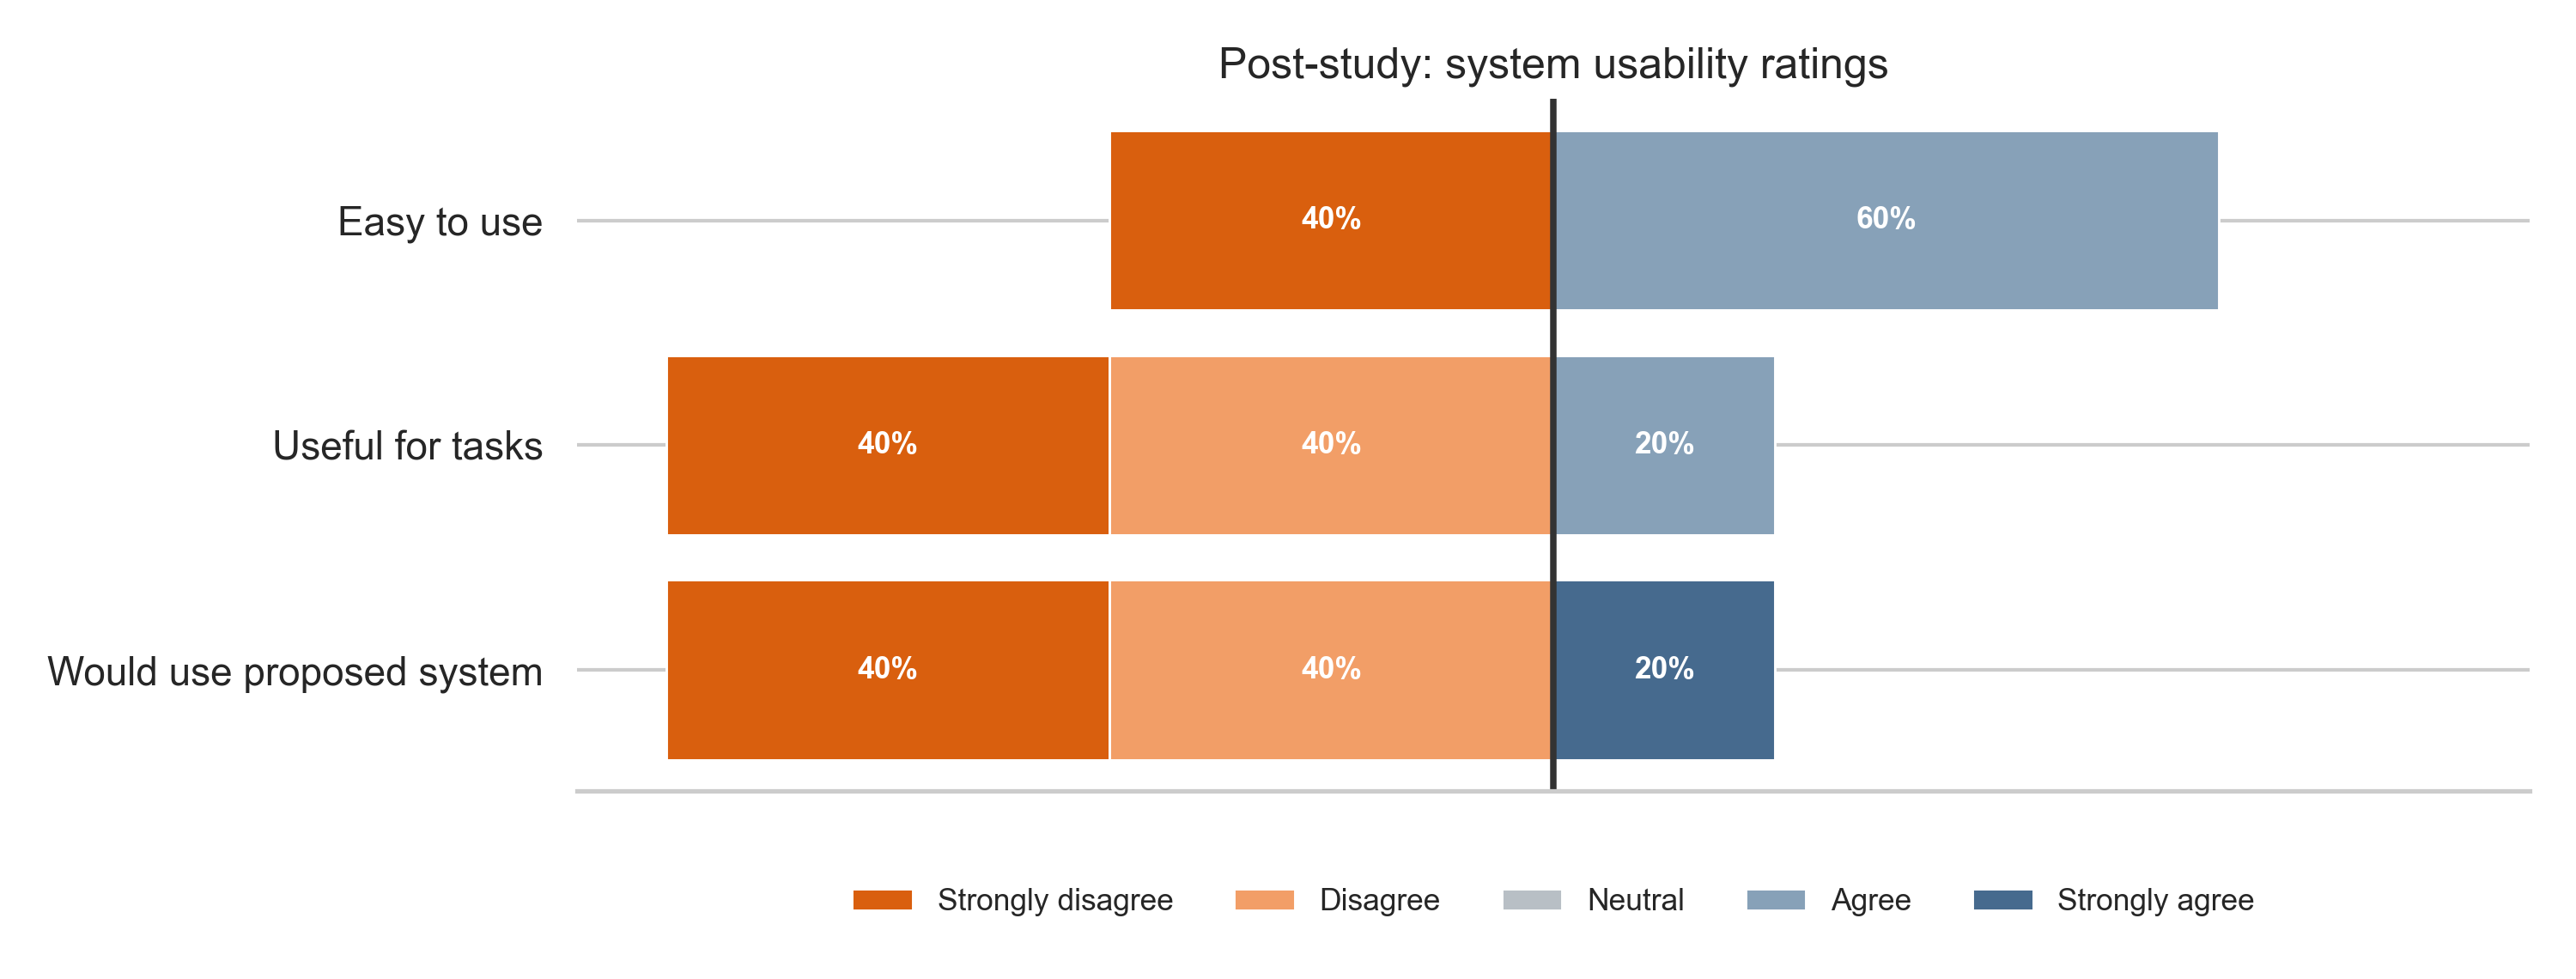
\includegraphics[width=\columnwidth]{media/evaluation/post_study_system_usability_diverging.png}
    \caption{Post-study system-usability ratings (ease of use, perceived usefulness, and willingness to use) shown as a divergent stacked Likert chart.}
    \label{fig:evaluation:post-study-system-usability}
\end{figure}

\subsection{Qualitative Findings}
Open-ended question responses and observations were consistent with the quantitative findings. The open-ended answers show that participants saw clear potential value in the proposed system, but only if it became more reliable and easier to use in practice. In the pre-study responses, participants mainly described AI assistance as useful for speeding up work, helping with drafts, and suggesting possible solutions. In the post-study responses, most participants said they would only use the system after further improvement, and several pointed to the same issues: wrong or irrelevant answers, slow responses, and a lack of direct guidance for changing the program files.

Participants also suggested a number of concrete improvements. The most common requests were for more direct help with the program files, such as line numbers, exact change locations, or code that could be copied into the file. Several participants asked for the system to work more closely with the current open program, to show the active file more clearly, or to add the program as context automatically. Others wanted clearer context handling, the ability to stop requests while the assistant is still working, and a more reliable search experience for discovering programs. Participants were generally not satisfied with the raw \texttt{.urpx} program format and a few suggested either representing programs like UR Studio or as URScript for at better experience.

The observation notes support these comments. Several participants expected the assistant to know the open program automatically, to show line numbers, or to edit the file more directly. Others found it hard to tell whether context had actually been added, or expected the added context to appear under their question rather than only in the assistant response. Some also tried actions that are natural in a file editor but not supported by the proposed system, such as using multiple cursors, and right-clicking or dragging program-tree nodes.

Across participants, the most frequent themes were:
\begin{itemize}
    \item \textbf{Context relevance issues:} Responses were often influenced by earlier prompts or unrelated retrieved context, which made them less useful for the current question. Participants described this as the assistant "remembering" the wrong thing or mixing in unrelated program details.
    \item \textbf{Mismatch between assistance and editing format:} Several responses described actions in the standard UR interface rather than concrete edits in the provided raw \texttt{.urpx} representation.
    \item \textbf{Insufficient actionability:} Participants repeatedly asked for line numbers, exact change locations, or code snippets that could be used directly. This was especially clear in the modification tasks, where the assistant often gave general advice instead of a precise edit.
    \item \textbf{Usability friction:} Participants reported that manual editing in the raw \texttt{.urpx} format is difficult and error-prone. The notes also show several small but important interface problems, such as unclear context attachment, a missing stop button, confusing chat history behavior, lost edits after switching tabs, and difficulty understanding whether context had been added correctly.
    \item \textbf{Performance concerns:} Participants noted that assistant responses were slow and practical barrier to using the system for real work.
\end{itemize}

Overall, the qualitative findings suggest that the general idea of AI assistance is accepted. However, the current implementation lacks quality and features. The main problems of the proposed system are that the assistant does not stay focused on the current query, does not give direct enough help for editing programs, and the program editing interface has several usability issues mentioned above.

